\chapter{Conclusion} % Main chapter title

\label{Chapter:Conclusion}

The complexities involved in the development of sustainable cities cannot be ignored by researchers and city authorities. The idea of sustainable city has over the years been simplified. Researchers and authorities focus mostly on the multi-functional dimensions of sustainability and overlook the complementary and conflicting roles of these functions. This report, which seeks to determine the relation between urban agriculture and sustainable cities, and a educational contribution through a mobile application (Garden Gem) has addressed various sustainable indicators in the sustainable city discourse. This report is based on a framework that takes into consideration the sustainability of cities from the economic, social and environmental sustainability dimensions.

The results show that the social, economic and environmental functions of urban agriculture have both positive and some negative outcomes. Moreover, the survey shows that more people are willing to engage in urban agricultural activities with the help of a mobile application, which provides basic agricultural educational information with the ability to track the produce progress. The report's analyses confirm, the benefits of urban agriculture especially the ecological and social dimensions have been ignored. Researchers such as Veenhuizen \cite{Veenhuizen} and Yamusa \cite{Agbenyour2014} argue that the contributions of urban agriculture to sustainable cities have been overestimated. Nevertheless, the analyses indicate that urban agriculture can drive development countries to sustainability.

Cities with large vacant lands, urban agriculture should be implemented with responsible integrations into the city land zoning planning. In the developed countries, ecologically sensitive regions can be protected to provide spaces for urban farming practices to reinforce the ecological functions. Nevertheless, in developing countries such as Ghana, urban agriculture can help to protect the ecologically sensitive areas. Responsible agriculture is required for the sustainable cities, which will aims to the protection of the ecological functions of urban gardens.

GardenGem will be a functional "plant data base" to allow the users to search over 30,000+ plants of the world over multiple criteria and get up-to-date information about their specific requirements for successful culture. GardenGem aims to become the most reliable resource for food education and urban agriculture development. After having provided the information and "know how" to the users, we will be adding hardware on sale for the physical improvement of their urban gardens. For this step, we will be contacting external providers to announce their products on our application and make them compatible with our technology. One of the main projects we are to be involved in is OpenAg Initiative from the MIT. The Personal Food Computer (PFC) they have developed has all the hardware and software design necessary for the automation of crops. (pfc\_edu\_3.0 OpenAg, 2019) Together with GardenGem, this computer may be more easily operated by any user. Talking with authorities to provide legal advice and permits in the development of this gardens in public areas is another important task to be done for a larger positive impact in local communities.


%\begin{figure}[th]
%\centering
%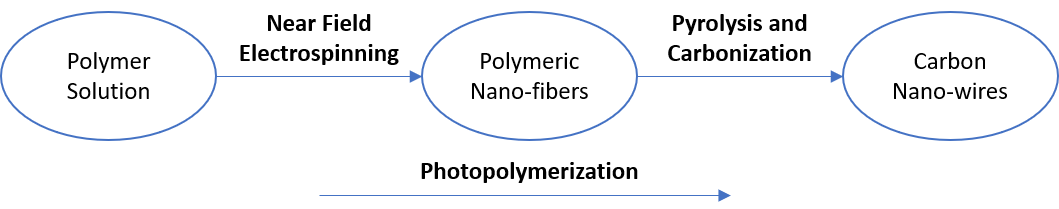
\includegraphics[width=0.95\textwidth]{./Figures/FabricationProcess.png}
%\decoRule
%\caption[Carbon Nano-wires Fabrication Process]{Fabrication process of carbon nano-wires to achieve through the proposed dissertation.}
%\label{fig:fabricationFlowChart}
%\end{figure}

%\begin{equation}
%\left(\tau _t^e-\frac{\tau _n^e \text{dr}}{\text{dz}}\right) 2 \pi  r+\frac{d \left(\pi  r^2
%   \left(\tau _{\text{zz}}-p\right)\right)}{\text{dz}}+\frac{\gamma  \text{dr} 2 \pi  r}{r
%   \text{dz}}+\rho  g \pi  r^2=\frac{d \left(\rho  \pi  r^2 v^2\right)}{\text{dz}}
%\label{eq:linearMomentum}
%\end{equation}